\documentclass[a4paper,oneside,11pt]{article}
\usepackage{graphicx}
\usepackage{ tipa }
\usepackage{hyperref}
\usepackage{titling}
\usepackage{blindtext}
\usepackage{enumitem}
\usepackage{eurosym}
\usepackage{float}
\usepackage{listings}
\usepackage{tabularx}
\usepackage{caption}
%\captionsetup[figure]{labelformat=empty}


\title{Requirements Analysis and Specification Document}
\author{Veljko Tatalović, Nikola Dimić, Edin Žiga}
\date{\today}
\begin{document}
    \begin{titlingpage} 
        \begin{center}
            
\includegraphics[height=5cm]{assets/Logo_Politecnico_Milano.png}\\
            \vspace{4cm}
            \begin{huge} 
                \textbf{\thetitle} \\
            \end{huge}
            \vspace{0.3cm}
            \begin{Large}
                \textit{Students \& Companies} \\
                \vspace{0.3cm}
                \textit{\today}
            \end{Large}
        \end{center}

            \vspace{4cm}
             \begin{large}
            \textbf{Authors:}
            \begin{itemize}
                \item Dimić Nikola
                \item Tatalović Veljko 
                \item Žiga Edin
            \end{itemize}
        \end{large}
    \end{titlingpage}
    \newpage
    \tableofcontents
    \newpage
    \section{Introduction}
    
        \subsection{Purpose}
            \quad The purpose of the Students \& Companies (S\&C) platform is to provide a centralized, user-friendly environment where university students can search for internship opportunities and where companies can advertise their offers. By consolidating internship advertisements in one place, the platform allows students to easily compare opportunities based on criteria such as required skills, offered benefits, and other terms. It ensures a safe and transparent process, minimizing the risk of exploitation by providing mechanisms for university supervision and feedback. Companies benefit from the platform’s reach, enabling them to connect with a broad pool of talented students efficiently. In addition, the platform fosters trust by ensuring university oversight, making it a reliable space for students and companies to interact.

\subsubsection{Goals}
\begin{itemize}
    \item \textbf{[G1]} Companies create internship advertisement.
    \item \textbf{[G2]} Students find appropriate internship and initiate contact with the selected company.
    \item \textbf{[G3]} Students become interns in the companies in order to gain experience in the desired area of industry.
    \item \textbf{[G4]} The platform provides a transparent and fair selection process where companies can evaluate and select suitable candidates.
    \item \textbf{[G5]} The platform offers a recommendation system that matches students to internships based on their CVs, skills, and preferences, as well as company requirements.
    \item \textbf{[G6]} The platform allows universities to monitor internships to ensure alignment with academic standards.
    \item \textbf{[G7]} The platform collects feedback from both students and companies to improve the platform’s functionality.
    \item \textbf{[G8]} Ensure a safe and supportive environment by providing students with mechanisms to file complaints and enabling universities to resolve them.
    
\end{itemize}
        \subsection{Scope}
            % To define the scope of the product we can use ``The World  \&  Machine'' approach by M. Jackson and P. Zave.
% We can define the real world entities that interact with the system (the World), the entities that belong to the system (the Machine) and the shared phenomena (the intersection of the two other sets).


The S\&C platform is designed to streamline the internship process by addressing the needs of three main user groups: Companies, Students, and Universities. Each group is provided with custom functionalities to support their respective roles in the internship ecosystem. \\

The platform enables companies to efficiently create and manage internship advertisements. These advertisements include detailed descriptions of requirements, projects, and relevant terms, ensuring clarity for prospective applicants. Companies can accept internship applications from students and handle the entire selection process, supported by tools for conducting interviews and distributing structured questionnaires. While the platform is conducting all the necessary steps in order to complete the selection process, interviews are supposed to be held on the external service (Microsoft Teams, Google Meets...) Once an internship is filled, companies are encouraged to provide feedback on their experience with the platform and its functionalities. \\

Students can utilize the platform to upload their data and CVs, creating comprehensive profiles that highlight their skills and experiences. They can search for internship opportunities that align with their goals and proactively initiate the application process. The platform enables easy and smooth participation in the selection process by allowing students to respond to invitations to interviews and questionnaires. In addition, students receive timely notifications regarding their selection status and are encouraged to provide feedback on their experience. For any challenges encountered during an internship, the platform provides a mechanism for students to submit complaints. \\

Universities play a crucial role in ensuring the integrity of the internship process by handling complaints submitted by students. They monitor and resolve issues, ensuring that internships provide a safe and productive environment. This oversight contributes to maintaining the reputation of the platform as a trusted intermediary between students and companies. Handling of the complaints should be done between the university, student, and company directly and not through the platform.

\subsubsection{World Phenomena}

\begin{itemize}
    \item \textbf{WP1} Students have their own CVs, experiences, and preferences when looking for internships.
    \item \textbf{WP2} Companies create internship opportunities and search for qualified candidates for their roles.
    \item \textbf{WP3} Company employees decide how the process of selection will look like before accessing the platform.
    \item \textbf{WP4} Complaints and conflicts can arise during internships, requiring resolution by a neutral entity (universities).
    \item \textbf{WP5?} Students participate in interviews and selection processes conducted by companies.
    
\end{itemize}

\subsubsection{Shared Phenomena}

\textbf{World controlled}
\begin{itemize}
    \item \textbf{SPW1} Students upload their CVs, experiences, projects and personal data.
    \item \textbf{SPW2} Companies interact with the system to upload internship advertisements and define the process of selection.
    \item \textbf{SPW3} Students use the system to search for internships and submit applications.
    \item \textbf{SPW4} Students and companies exchange information through the platform, including interview schedules and questionnaires.
    \item \textbf{SPW5} Companies evaluate students who went through the selection process and mark the selected ones.
    \item \textbf{SPW6} Students that got accepted decide whether they want to enroll the selected internship
    \item \textbf{SPW7} Universities use the system to access complaints submitted by students and monitor internship progress.
    
\end{itemize}
\textbf{Machine controlled}
\begin{itemize}    
    \item \textbf{SPM1} The system recommends internships to students based on their CVs, projects and preferences
    \item \textbf{SPM2} Notifications about new internships or application statuses are automatically sent to users.
    \item \textbf{SPM3} The system requests for feedback and ratings from both students and companies, contributing to platform analytics and recommendations.
    \item \textbf{SPM4} The platform provides suggestions to students and companies to improve their CVs or internship postings, based on statistical and user feedback.
    \item \textbf{SPM5} The system tracks and records complaints submitted by students and sends them to universities.
\end{itemize}

\subsubsection{Machine Phenomena}
\begin{itemize}
    \item \textbf{MP1} The system stores and processes student profiles, including CVs and other personal data.
    \item \textbf{MP2} The system contains a searchable database of internship advertisements.
\end{itemize}



        \subsection{Definitions, Acronyms, Abbreviations}
            \renewcommand{\arraystretch}{1.5}
\subsubsection{Definitions}
\subsubsection{Acronyms}
\begin{itemize}
    \item S\&C: Students\&Companies;
    \item UI: User Interface;
    \item UML: Unified Modeling Language.
\end{itemize}
\subsubsection{Abbreviations}
\begin{itemize}
    \item G*: goal
    \item WP*: world phenomena
    \item SP*: shared phenomena
    \item R*: functional requirement
    \item UC*: use case
\end{itemize}
        \subsection{Revision history}
         \textbf{v1.0} - 7/12/2024 - Initial release \\


        \subsection{Reference documents}
            This document is based on the following:
\begin{itemize}
    \item The specification of the RASD and DD assignment of the Software Engineering II course;
    \item Slides of Software Engineering II course on WeBeep;
    \item Larman, C. (2002). Applying UML and patterns: An introduction to object-oriented analysis and design and the Unified Process. Prentice Hall PTR. 
\end{itemize}
        \subsection{Document structure}
        \renewcommand{\arraystretch}{1.6}
This RASD document consists of the following parts:
\begin{enumerate}
    \item \textbf{Introduction}: It aims to give a brief description of the project. In particular
    it’s focused on the reasons and the goals that are going to be achieved with its
    development;
    \item \textbf{Overall Description}: it is an high-level description of how the system works with
    a detailed explanation of the phenomena that involve the world, the machine or
    both;
    \item \textbf{Specific Requirements}: in this section there is a detailed analysis of the requirements
    needed to achieve the goals. Moreover, it contains more information useful for
    developers;
    \item \textbf{Formal analysis}: it’s a formal description of the world phenomena by the means
    of Alloy;
    \item \textbf{Effort spent}: it shows the time spent to realize this document organized by section;
    \item \textbf{References}: it contains the references to any documents and software used to write
    this paper.
\end{enumerate}
        
    \newpage
    \section{Overall Description}
        \subsection{Product perspective}
            \subsubsection{Scenarios}

\quad \textbf{User creates an account on the platform}\\ 
Two main users of the platform have to create an account (companies and students). Company has to provide all the information relevant for the company, while student uploads their CV and other relevant information to create a profile that showcases their skills and experiences.\\

\textbf{Company creates an internship advertisement}\\
A company access the platform using their credentials and selects an option to create an internship advertisement. After opening the page for creation of the advertisement, the platform requires detailed internship description, specifying required skills, project descriptions, offered benefits, and application instructions. Also, the company must define how will the selection process look like (e.g. if there will be more then one interview, questionnaire or more than one round of selection process)  \\

\textbf{Company manages internship advertisements}\\
Anytime, a company has an option on the platform to manage active internship advertisements. A company has possibility to update or remove an existing advertisement, ensuring it reflects the latest requirements or availability.\\

\textbf{Student searches and applies for internship opportunities }\\
A student after logging in with his credentials on the platform, the home page is populated with the active internship advertisements which one can browse, filtering by location, required skills, or other criteria. After finding and selecting appropriate internship, the platform opens page with the detailed description, requirements and other information about the internship. Student has an option to apply for the selected internship.\\

\textbf{Company reviews student applications}\\
A company, on their profile can view student applications for every active internship advertisement. The company can evaluate every student's suitability based on uploaded CV, skills and preferences. The platform provides an option for the applied students to accept and continue with the selection process as the company has chosen in the creation of the advertisement, or reject student if they believe they are not right fit for the company. After the acceptance of the certain students, the company has an option to send them questionnaire. \\

\textbf{Student participates in the selection process}\\
After the company selects the student to continue with the selection process, the student receives a notification and has an option to complete a questionnaire provided by a company. The student submits filled questionnaire and waits for the company to send him an invitation for the interview. During the selection process, student has an option to see his progress and all the rounds he has to pass in order to finish the selection process (e.g., questionnaire completed, interview completed).\\

\textbf{User provides feedback on the platform}\\
After the internship concludes, users will get a feedback questionnaire from the platform in order to collect statistical data and improve the recommendation system. The company has to provide feedback about the student’s performance and the platform’s usefulness, while the student has to give some insights about the internship and the company that he worked for.\\

\textbf{The platform recommends internships to students}\\
The recommendation system integrated in the platform recommends internships to the student based on his projects, CV and relevant data that the student uploaded when creating an account. The recommendation system analyzes a student’s profile and suggests internships that match their skills, experiences, and preferences. The recommendation system utilizes simple keyword searching in order to match the internships that could be related to the student's portfolio. \\

\textbf{User submits a complaint to the platform}\\\
During the internship, both the student and the company can file a complaint about issues that can arise. Both users have an option on the platform to file a complaint on the active or completed internship. The platform handles the complaint further. \\

\textbf{University reviews and handles complaints}\\
After the complaint has been filled, the university gets a notification about an active complaint request with all the information that user mentioned. The university communicates with the company and the student to resolve the issue, potentially leading to corrective actions or termination of the internship. If the university decides that the company has not met the benefits and requirements that were mentioned in the internship advertisement, the university can request from the platform to forbid internships from that company to its students.\\

\textbf{University monitors internship progress}\\
The university has an option to monitor the internship progress through feedback related to ongoing internships to ensure compliance with academic and ethical standards. Also, the university has an option to monitor an active internship in order to assign the points to the student in the case of an obligatory internship. \\

%\textbf{Student receives notifications for new internships}\\
%The platform notifies a student about newly added internships that match their profile and preferences.\\

%\textbf{Company conducts interviews via the platform}\\
%A company schedules and conducts interviews with candidates through integrated video calls or other system-%supported methods.\\

%\textbf{Company finalizes candidate selection}\\
%A company selects the most suitable candidate(s) for the internship and sends a confirmation through the platform.\\

\subsubsection{Domain class diagram}

\quad The domain class diagram for the S\&C platform is presented in figure x.x. It is designed to represent all major entities and relationships described in the scenarios. The User class serves as a base class for Student, Company, and University which extend it. It encapsulates common attributes. Each subclass adds specific details needed for each role, such as CV and preferences for students, companyName and description for companies, and universityName for universities. Other key classes include InternshipAdvertisement for managing detailed internship postings, InternshipApplication for tracking application statuses, and Complaint for handling issues raised by users. Additional classes like Recommendation and Feedback enhance platform functionality by supporting personalized internship suggestions and collecting user feedback. \\

The relationships between these classes reflect real-world interactions. For instance, companies create and manage InternshipAdvertisement objects, which are linked to multiple InternshipApplication objects submitted by students. The Recommendation class associates student profiles with internships using criteria (e.g. skills and preferences). Both students and companies can provide Feedback about internships and file Complaint objects for university review. Universities handle complaints, monitor internships through the InternshipMonitoring class, and ensure compliance with academic standards.
%These relationships and associations provide all the functionalities on the platform, from internship advertisement creation to application management, selection processes, and complaint resolution. \\

%This design emphasizes scalability, maintainability, and data integrity. Its modular structure supports future feature expansion, such as additional user roles or advanced recommendation algorithms. By separating responsibilities among students, companies, and universities, the system ensures clarity and efficiency. Strong associations between classes enforce data consistency, while role-specific features improve usability for all stakeholders. Overall, the diagram provides a comprehensive foundation for implementing the S\&C platform.


\subsubsection{State diagrams}

\quad This section is going to visually present lifecycle of different components on the platform using state diagrams. Following state diagrams are covering management of internship advertisement, internship application and complaint handling. \\

\textbf{Internship advertisement management}\\
\begin{figure}[H]
	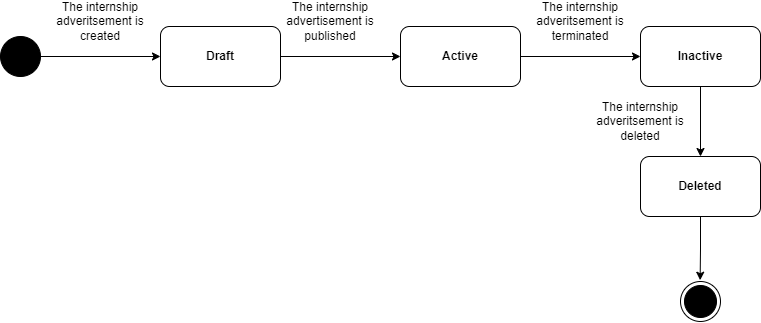
\includegraphics[width=\textwidth,height=\textheight,keepaspectratio]{RASD-Latex/assets/state_diagram.png}
	\caption{Internship advertisement state diagram}
	\label{fig:DataRequest}
\end{figure}

This diagram represents the lifecycle of an internship advertisement on the platform, focusing on states like \textit{Draft}, \textit{Active}, \textit{Inactive}, and \textit{Deleted}. Internship advertisement lifecycle starts from the state \textit{Draft}. This is the initial state when a company starts creating an internship advertisement until it is published. Companies can add details such as required skills, project descriptions, and selection processes. Once the advertisement is finalized and submitted, it transitions to the \textit{Active} state. Active advertisements are visible to students, allowing them to search and apply. The advertisement can be marked as inactive by the company if it's no longer available or requires updates. Inactive advertisements are not visible to students. If the advertisement is no longer needed, it transitions to the \textit{Deleted} state. Deleted advertisements are permanently removed from the platform. Transitions between these states occur based on user actions.\\

\textbf{Internship application management}\\
\begin{figure}[H]
	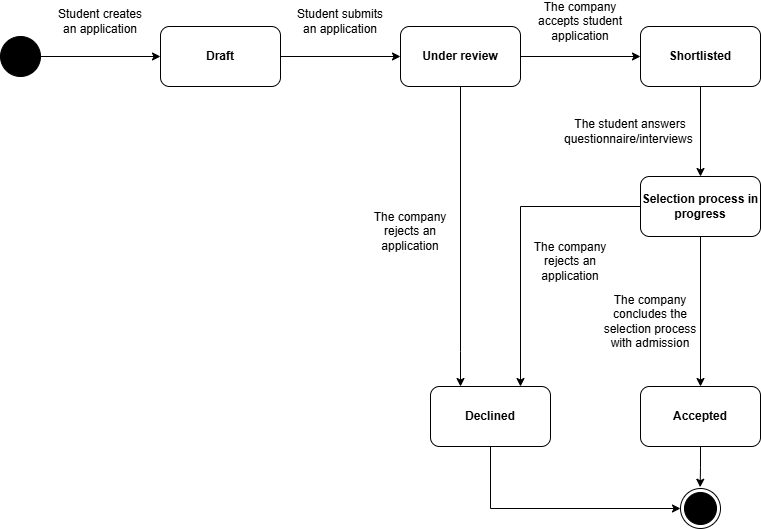
\includegraphics[width=\textwidth,height=\textheight,keepaspectratio]{RASD-Latex/assets/state_diagram_2.png}
	\caption{Internship application state diagram}
	\label{fig:DataRequest}
\end{figure}

Application and selection process for students and companies are showed in the state diagram above (figure x.x). After a student applies for an internship, their application enters the \textit{Under Review} state. The company evaluates the application based on the CV and profile. If the student’s application meets the company’s criteria, it transitions to the \textit{Shortlisted} state. The student is notified of their progress. After shortlisting, the selection process begins. This could involve questionnaires, interviews, or other methods defined by the company. The platform keeps track of the student's progress through each stage. If the student is not a fit, their application transitions to the \textit{Declined} state with the reason for that decision indicated by the company. The student is notified of the rejection. On the other hand, if the student successfully completes all selection stages, their application moves to the \textit{Accepted} state. This indicates that the student has secured the internship. \\

\textbf{Complaint management}\\
\begin{figure}[H]
	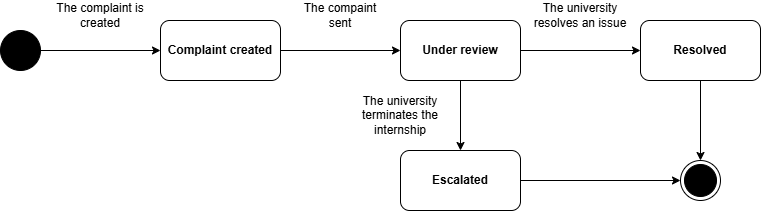
\includegraphics[width=\textwidth,height=\textheight,keepaspectratio]{RASD-Latex/assets/state_diagram_3.png}
	\caption{Complaint handling state diagram}
	\label{fig:DataRequest}
\end{figure}

The complaint process starts when a user (student or company) creates a complaint. The complaint moves to the state \textit{Complaint created}. Immediately, the next state \textit{Under review} is active. In that state, the university begins the review process. In this state, the university evaluates the complaint, gathering information from involved parties (e.g., students, companies, or both). If the issue cannot be resolved, the university has an option to terminate the internship and in that case state is \textit{Escalated}. Whereas, if the university successfully resolves the complaint, complaint process transitions to the \textit{Resolved} state.




        \subsection{Product functions}
            \textbf{User Registration and Authentication} \\
The platform allows students, companies, and universities to register by creating accounts and logging in using secure authentication methods. Users can register by pressing the button "Sign up" and the platform will send them on the registration page where they will enter necessary data. Students provide their CV and skills, companies enter relevant business information, and universities add institutional details. This ensures that all users are identified and role-specific functionalities are enabled. If the user is already registered on the platform, there is an option to login using user credentials. \\

\textbf{Profile Management} \\
Each user can manage their profiles by updating personal information. The platform offers the page with the possibility of viewing data of the logged in user and modifying it. Students can upload and update their CVs, skills, and preferences; companies can refine their organizational descriptions; and universities can manage their institutional profiles. This enables users to keep their information relevant and up-to-date. \\

\textbf{Internship Advertisement Creation and Management} \\
Companies are able to access the page for advertisement creation by pressing the button "Create new internship advertisement" where they can create internship advertisements by providing detailed information about the role, required skills, offered benefits, and the selection process. In addition, there is an option to view all active internship advertisements, where they can be updated, activated, deactivated, or deleted to ensure only relevant opportunities are visible to students. \\

\textbf{Internship Search and Application} \\
The platform offers students possibility to search for internships using filters like location, required skills, and benefits. They can view detailed descriptions of each internship by pressing on the box where the advertisement is located. After pressing on the selected advertisement the platform sends user on the page where details of the internship are presented. Button "Apply" is located on the internship page. That way, student can submit application directly through the platform. \\

\textbf{Selection Process Management} \\
On the company user page on the platform, company can view the status of any student that is in the selection process. The company can distribute and view the questionnaire that the student answered, schedule an interview with the student, view the date and time of scheduled interview and also can terminate the selection process anytime if decides that the student is not right fit for the internship role, with giving the reason for such decision. On the other hand, the student that is in the active selection process can view their progress, view the questionnaire and the deadline for submitting it. As the company, the student can view the date and time of the scheduled interview. \\

\textbf{Feedback System} \\
Feedback system which is integrated on the platform is responsible for collecting information from the students and companies after the selection process finishes and after the internships conclude. Companies provide feedback on the students’ performance and their experience using the platform, while students share their thoughts about the platform or about the internship and the company. Data collected this way is used for improvement of the platform and in order to build trust between users. \\

\textbf{Recommendation System} \\
The recommendation system is built with the intention to suggest internships to students based on their CVs, skills, and preferences. Method that the recommendation system uses is  a keyword-matching algorithm to identify opportunities that align with a student’s profile, helping them find relevant internships more efficiently. On the home page of the platform when the logged in user is student where the internship opportunities are shown, the first one which are showed are the ones that recommendation system chose. Those internship advertisements have label \textit{Suggested} in order to highlight them.\\

\textbf{Complaint Handling System} \\
Both students and companies can submit complaints about issues that arise during selection process or internships that are active or completed. The platform provides an option on the page of the active internship or selection process to file a complaint. Complaints are reviewed by universities, which act as mediators to resolve disputes. When the complaint is requested by the student or the company, the university account gets a notification about the active complaint request. This system ensures that the platform maintains ethical and fair practices. \\
%Add how is the complaint handled by the university??

\textbf{Internship Monitoring}\\
Universities are able to monitor ongoing internships by accessing feedback and progress reports. Progress reports are requested for the student and the company every month. This function ensures compliance with academic and ethical standards. This way universities can monitor the internship progress and assign points to students for completed internships when required. \\

\textbf{Notifications System} \\
The platform is equipped with the notification system which sends notifications to students and companies at various stages, such as when new internships are posted, application statuses are updated, or when students are invited to the next step in the selection process. Notifications keep users informed and engaged. \\


        \subsection{User Characteristics}
            Users that are present on the platform and interact are: \textit{Student}, \textit{Company} and \textit{University}.

\subsubsection{Student}
User \textit{Student} has an option to sign up and login in order to access the platform. On the platform the student can search for the internships and apply for them. The student can be shortlisted or declined. If the student is shortlisted, he continues with the selection process which results with admission to the internship or rejection. The student has a possibility to file a complaint if the selection process or an active internship is not as described in the advertisement or are not by academic or ethical practices.


\subsubsection{Company}

User \textit{Company} is, as the student, can sign up and login in order to access the platform. When logged in, the company can create and manage an advertisement for an internship role that is open. Company is able to manage the selection process and guide students through it. Also, the company may file a complaint if the internship progress is not as expected due to student misbehaviour. 



\subsubsection{University}
User \textit{University} is responsible for monitoring and supervising the process of selection and progress of the active internships. The university user are able to sign up and log in to the platform. In addition, this user has to handle complaint requests by students and companies. 


        \subsection{Assumptions, dependencies and constraints}
            \subsubsection{Regulatory policies}

The S\&C platform operates within the framework of applicable local laws and regulations about employment and internships. It follows labor laws that protect interns from exploitation in Italy, ensuring fair compensation and working conditions. The platform complies with data protection regulations, such as GDPR, by securing user data and limiting access to authorized personnel. Companies must ensure that the internships meet employment standards and are according to anti-discrimination policies. Universities play a regulatory role by monitoring internships to ensure ethical practices and compliance with academic requirements.
%Change the text a little bit??

\subsubsection{Domain assumptions}

The following domain assumptions are needed in order for the platform to work successfully. 

\begin{itemize}
    \item \textbf{[D1]} User must have a reliable internet connection.
    \item \textbf{[D2]} All users provide accurate information when creating profiles.
    \item \textbf{[D3]} Universities actively engage with the platform in order to monitor active internships and to resolve complaints.
    \item \textbf{[D4]} Companies provide accurate information about an internship.
    \item \textbf{[D5]} The system will be available ensuring uninterrupted access to users.
    \item \textbf{[D6]} Submitted complaints are genuine and not misused to create unnecessary conflicts.
    \item \textbf{[D7]} Companies respond to applications promptly.
    \item \textbf{[D8]} Students complete selection process steps within deadlines.
\end{itemize}

    \newpage
    \section{Specific Requirements}
        \subsection{External Interface Requirements}
            \subsubsection{User Interfaces}
\subsubsection{Hardware Interfaces}
While the platform is primarily a web application, specific hardware requirements exist to fully utilize all available features.

The minimum requirement for accessing and using the platform is a keyboard and a device that supports a modern browser compliant with HTML5 standards, as the user interface will comply with keyboard accessibility standards outlined in the Web Content Accessibility Guidelines (WCAG) 2.1.

Although not mandatory, using a pointing device is encouraged for efficiency. No specific pointer device is required for PCs or mobile devices, as the HID protocol and touchscreens are widely supported.

As the platform will support multi-factor authentication (MFA), users are encouraged (but not required) to possess an external iOS- or Android-based mobile device for this feature. MFA will be supported through an authenticator app and/or passkeys.

Passkeys can be configured using in-built fingerprint readers and/or face-ID scanners on mobile devices. Therefore, users will need a fingerprint- or face-ID-enabled mobile device to configure and use passkeys.

Lastly, the platform will allow users to register a FIDO2/WebAuthn-compliant hardware authenticator (e.g., from Yubico). To use this feature, users must possess the hardware authenticator as well as either an NFC-enabled mobile device or an HID-compliant USB port on any platform.

A summary of the described hardware interfaces is provided below.

\paragraph{Mandatory Hardware Interface Requirements (MHIR)}
\begin{itemize}
    \item \textbf{MHIR1.} An HID-compliant keyboard
\end{itemize}

\paragraph{Recommended Hardware Interface Requirements (RHIR)}
\begin{itemize}
    \item \textbf{RHIR1.} An HID-compliant pointer device
    \item \textbf{RHIR2.} A fingerprint- or face-ID-enabled mobile device
\end{itemize}

\paragraph{Optional Hardware Interface Requirements (OHIR)}
\begin{itemize}
    \item \textbf{OHIR1.} A FIDO2/WebAuthn-compliant hardware authenticator
    \item \textbf{OHIR2.} An NFC-enabled smartphone
    \item \textbf{OHIR3.} A device with an HID-compliant USB port
\end{itemize}


\subsubsection{Software Interfaces}

As noted, in order for the application to be accessed, it must be done through a modern, HTML5-compliant browser, regardless of the operating system or browser type. 

The platform will be fully hosted on Amazon Web Services (AWS), so access to specific AWS APIs (e.g., AWS S3, AWS Lambda) and their associated endpoints will be required for its proper functionality. Additionally, the MFA feature will utilize the Time-Based One-Time Password (TOTP) API.

Furthermore, as part of the platform's Artificial Intelligence (AI) integration to enhance user profiles, the OpenAI ChatGPT API will be employed. For legacy system compatibility (e.g., older authentication methods), additional APIs will also be included to ensure backward compatibility.

The platform may also support additional MFA methods, such as SMS-based codes or hardware tokens, to accommodate different user preferences.

A summary of the described software interfaces is provided below.

\paragraph{Mandatory Software Interface Requirements (MSIR)}
\begin{itemize}
    \item \textbf{MSIR1.} A modern, Web2-compliant browser
    \item \textbf{MSIR2.} AWS API and subsequent endpoints (e.g., AWS S3, AWS Lambda)
    \item \textbf{MSIR3.} OpenAI ChatGPT API
    \item \textbf{MSIR4.} WebAuthn for FIDO2 authentication
    \item \textbf{MSIR5.} U2F (Universal 2nd Factor), a legacy FIDO protocol for second-factor authentication
    \item \textbf{MSIR6.} TOTP API for generating one-time passwords
    \item \textbf{MSIR7.} Twilio or Nexmo API for sending SMS-based one-time passcodes
    \item \textbf{MSIR8.} OATH OTP algorithm or FIDO2/WebAuthn for hardware token-based authentication
     \item \textbf{MSIR9.} Add AntiMalware API here

\end{itemize}




\subsubsection{Communication Interfaces}
The primary means of communication between the web application and the various backend systems as well as external services will invlove HTTPS protocols, RESTful APIs and various WebSocket connections where required. 


        \subsection{Functional Requirements}
            

\newcounter{reqCounter} % Define a custom counter for functional requirements
\stepcounter{reqCounter}

Within this section can be found a list of functional requirements for S\&C, categorized by the major features of the platform.

\paragraph{Registration of Students}
\begin{itemize}[label={[\textbf{FR\arabic{reqCounter}}]}, align=left, leftmargin=*]
    \item \stepcounter{reqCounter} The system shall allow new student users to register on the platform using their respective institutional accounts.
    \item \stepcounter{reqCounter} After an institutional account has been linked with the platform, the system shall allow student users to log in using their institutional credentials.
    \item \stepcounter{reqCounter} The system shall allow the registration of student users only if they are classified as students within the institutional account they provide.
\end{itemize}

\paragraph{Registration of Companies}
\begin{itemize}[label={[\textbf{FR\arabic{reqCounter}}]}, align=left, leftmargin=*]
    \item \stepcounter{reqCounter} The system shall allow new company users to register on the platform using a valid email address.
    \item \stepcounter{reqCounter} After providing an email address, the system shall verify the provided address through a verification email.
    \item \stepcounter{reqCounter} After the new company user has verified their email, the system shall generate and deliver a password for the newly created account via the verified email.
    \item \stepcounter{reqCounter} The system shall allow the company user to log in using the validated email address and the provided password.
    \item \stepcounter{reqCounter} Upon the first login, the system shall require the new user to provide a certificate from the relevant tax authority, including the company name and unique identifier. The system shall also require the full company name and unique identifier to be entered manually in the relevant input fields alongside the certificate.
    \item \stepcounter{reqCounter} The system shall retain company user data only at two points: first, after successful email verification, where the provided email address and generated password will be retained as login credentials; and second, after submitting the initial verification information, where all submitted data up to that point shall be retained.
\end{itemize}



\paragraph{Registration of Universities}
\begin{itemize}[label={[\textbf{FR\arabic{reqCounter}}]}, align=left, leftmargin=*]
    \item \stepcounter{reqCounter} The system shall allow new university users to register on the platform using pre-designated institutional accounts allocated for S\&C.
    \item \stepcounter{reqCounter} After an institutional account has been linked with the platform, the system shall allow university users to log in using their institutional credentials.
    \item \stepcounter{reqCounter} If the institutional account has not been pre-designated for use on S\&C, the system shall reject the registration attempt.
\end{itemize}

\paragraph{Profile Management}
\begin{itemize}[label={[\textbf{FR\arabic{reqCounter}}]}, align=left, leftmargin=*]
    \item \stepcounter{reqCounter} The system shall, by default, provide a blank profile template for all users.
    \item \stepcounter{reqCounter} The system shall provide different collections of predetermined fields based on the user type.
    \item \stepcounter{reqCounter} The system shall allow all users to edit each field in their profile, with the exception of unique identifiers, such as tax numbers for companies and universities, and unique IDs for students, which cannot be altered.
    \item \stepcounter{reqCounter} The system shall allow each field to be configured as public or private, provided that data is present in the respective field.
    \item \stepcounter{reqCounter} The system shall automatically configure all fields with no data as private.
    \item \stepcounter{reqCounter} The system shall allow all users to provide public hyperlinks to other platforms which the system shall display in a format that clearly indicates the platform to which the hyperlink leads to.
    \item \stepcounter{reqCounter} The system shall integrate OpenAI's ChatGPT 4.0 API into each field to provide AI-generated suggestions for profile improvements.
\end{itemize}



\paragraph{Internship Advertisement Creation and Management}
\begin{itemize}[label={[\textbf{FR\arabic{reqCounter}}]}, align=left, leftmargin=*]
    \item \stepcounter{reqCounter} The system shall only allow company users whose data has been verified to create, update, and delete public internship advertisements, where the system shall save unfinished advertisements as draft.
    \item \stepcounter{reqCounter} The system shall allow the creation of new internship advertisements only if they possess the following fields: name, internship duration, short description, location, internship type, and the number of stages in the application process.
    \item \stepcounter{reqCounter} The system shall integrate OpenAI's ChatGPT 4.0 API into each field of the internship advertisement creation process to provide AI-generated suggestions for enhancing the advertisement.
    \item \stepcounter{reqCounter} The system shall allow for numerous types of stages to be created, including but not limited to questionnaires and video interviews, which may be scheduled on external platforms.
   
    \item \stepcounter{reqCounter} Should the internship creation process be interrupted at any stage, the system shall save the unfinished internship advertisement as a draft.
    \item \stepcounter{reqCounter} After creation, the system shall allow company users to make updates to all fields of each internship advertisement they have created, with the exception of that internship advertisement's unique ID and publication timestamp.
\end{itemize}

\paragraph{Internship Search, Application, and Management of Applications}
\begin{itemize}[label={[\textbf{FR\arabic{reqCounter}}]}, align=left, leftmargin=*]
    \item \stepcounter{reqCounter} The system shall analyze the profile of the student user upon login and recommend 3 internship advertisements based on matching qualifications and background, and display these recommendations prominently to the student user.
    \item \stepcounter{reqCounter} The system shall allow student and university users to view all internship advertisements posted by any company on the platform, not just those they are applying to. Company users, however, will only be allowed to view and manage the advertisements they have created.
    \item \stepcounter{reqCounter} The system shall allow all student users to apply to internship advertisements, after which their profiles will be automatically inserted into the list of applicants under the Stage 1 category.
    \item \stepcounter{reqCounter} Upon a successfully submitted application, the system shall notify the advertisement's creator.
    \item \stepcounter{reqCounter} The system shall only allow company users who are creators of the internship advertisement to move candidates further along the selection stages.
    \item \stepcounter{reqCounter} The system shall allow the company user, at any given stage, to reject any candidate without mandating a reason.
    \item \stepcounter{reqCounter} Upon a change in status, be it a rejection or a move up in the selection stages, the system shall always notify the candidate of the change.
    \item \stepcounter{reqCounter} Upon reaching the final stage as designated by the company, the system shall automatically classify the candidate as accepted for the internship.
    \item \stepcounter{reqCounter} The system shall allow the company user to request the commencement of an internship from the candidate's host university. After the internship is approved by the host university, it shall commence on a predetermined date.
\end{itemize}

\paragraph{Internship Monitoring \& Complaint Management}
\begin{itemize}[label={[\textbf{FR\arabic{reqCounter}}]}, align=left, leftmargin=*]
    \item \stepcounter{reqCounter} During any stage of the internship, the system shall allow both the candidate and the company user to submit a complaint to the host university, after which the university user shall be automatically notified.
    \item \stepcounter{reqCounter} After a complaint is received, the university may choose to resolve the complaint or to terminate the internship. The system shall allow for both choices to be submitted.
    \item \stepcounter{reqCounter} The system shall not allow the termination of an internship by any party except the university user. The system shall allow a termination only after a complaint has been submitted.
\end{itemize}

% Ovo su NFRs koje sam izfiltrirao iz orginalnih FRs, koje cu dodat kasnije. Ovdje stoje samo kao note.
% \paragraph{NFRs}
% \begin{itemize}[label={[\textbf{FR\arabic{reqCounter}}]}, align=left, leftmargin=*]
%     \item \stepcounter{reqCounter} The system shall not retain any user data unless the student user registration process is fully completed.
%     \item \stepcounter{reqCounter} For company validation, the system shall exclusively accept files in the .pdf format for the initial company verification document. The system shall validate the file format and ensure that the file size does not exceed 10 MB.
%     \item \stepcounter{reqCounter} The system shall not retain any user data unless the registration process is fully completed. - Uni registartion
%     \item \stepcounter{reqCounter} The system shall take snapshots every 10 seconds during the internship advertisement creation process, where all filled fields will be saved. - Ad creation
%     \item \stepcounter{reqCounter} A submitted complaint has a maximum waiting period of 14 calendar days, after which the system shall automatically terminate the internship.
%     \item \stepcounter{reqCounter} The system shall automatically filter all text inserted in user fields for profanities. - Profile Management
%     \item \stepcounter{reqCounter} After the new company user has verified their email, the system shall generate and deliver a password with a minimum length of 32 characters, including a randomized combination of uppercase letters, lowercase letters, numbers, and special characters, for the newly created account via the verified email.
%     \item \stepcounter{reqCounter} The system shall ensure that the input field accepts only string-type inputs, with all Unicode characters supported. The system shall validate the input in real-time and reject non-string data types.
%     \item \stepcounter{reqCounter} Unless otherwise specified by the company, the system shall, by default, assign a 21-calendar-day duration for which the advertisement will be publicly viewable.
%     \item \stepcounter{reqCounter} The system shall not allow advertisements to be visible for more than 90 calendar days.
%     \item \stepcounter{reqCounter} The system shall, by default, provide the internship advertisements in batches of 10, with the most recent advertisements presented at the top of the list.
%     \item \stepcounter{reqCounter} The system shall provide an appropriate error message if the registration process is interrupted at any stage, specifying the reason for the interruption.
%     \item \stepcounter{reqCounter} The system shall provide an appropriate error message if the registration process is interrupted at any stage, specifying the reason for the interruption.
%     \item \stepcounter{reqCounter} The system shall provide an appropriate error message if the process is interrupted at any stage, specifying the reason for the interruption. The level of data retention will depend on the stage the user has reached before the interruption, as specified in [FR13].
% \end{itemize}




\subsubsection{Use cases Diagram}
\subsubsection{Use cases}
\subsubsection{Requirement mapping}

        \subsection{Performance Requirements}
            Performance requrements text

        \subsection{Design Constraints}
            Design contraints text

        \subsection{Software System Attributes}
            \subsubsection{Reliability}
During development, the entire platform will be subject to rigorous testing to ensure that all features are working as described with no variations. Moreover, as the application will be dockerized and deployed using AWS, it should ensure that should whichever instance of the platform experience issues, a new instance can be deployed instantly (should it be needed). 
\subsubsection{Availability}
Deploying on AWS ensures an availability metric between 99.80\% and 99.99\% (Amazon, 2024), even with issues such as cyber attacks or platform updates. As mentioned, most user activities will be subject to snapshots and draft-saving, hence, in the unlikely event of the platform going offline, users will be able to return to their activities precisely where they left off.
\subsubsection{Security}
Beyond following all the necessary privacy laws, the platform shall follow the highest possible security standards along with best practices as three different user groups with extremely sensitive data are at stake. Multi Factor Authentication shall be mandatory for all users and to end data encryption will be a minimum for all users, strong measures against data scraping shall be taken, a zero-trust architecture will be employed, and privacy by design will be the standard moving forward.
\subsubsection{Maintainability}
The software platform will be subject to the use of extensive testing and code analysis software. Technical debt shall be avoided at all costs, and monthly refactoring shall be a regular occurrence. Moreover, atomicity shall be forced for each software component, with test coverage being at 95\% at all time without exception.
\subsubsection{Portability}
S\&C is designed to be cross-platform, allowing access from virtually any device capable of processing JavaScript. In terms of porting the system to a different service provider, or moving to private hosting - the platform will benefit heavily from containerization and virtualization, therefore, transferring the client side application as well as any backend functionality to any other service should not prove to be an issue. Moreover, as identical backups of the database shall be created in real-time, migrating the database will be a straight-forward process with graceful database migration.


    \section{Formal analysis}
        \input{}

    \newpage

    \section{Effort spent}
        The time tables written below represent an approximation of the effort spent for the
creating each specific section of this document. These times for producing this document are based on the personal perception of the team members.

\begin{table}[h!]
\centering
\begin{tabular}{|l|c|c|c|c|c|}
\hline
\textbf{Student} & \textbf{Section 1} & \textbf{Section 2} & \textbf{Section 3} & \textbf{Section 4} & \textbf{Total Hours} \\ \hline
Veljko Tatalovic & 10 & 21 & 5 & 4 & 40 \\ \hline
Edin Ziga & 2 & 4 & 32 & 3 & 41 \\ \hline
Nikola Dimic & 7 & 8 & 7 & 18 & 40 \\ \hline
\end{tabular}
\caption{Effort Spent by students}
\label{tab:effort_table}
\end{table}
            
\end{document}